\documentclass[problem]{mcs}

\begin{pcomments}
  \pcomment{MQ_basic_network_problem}
  \pcomment{from: S09.ps7}
\end{pcomments}

\pkeywords{
  networks
  congestion
  input_output
  routing
  shortest_path_routing
}

%%%%%%%%%%%%%%%%%%%%%%%%%%%%%%%%%%%%%%%%%%%%%%%%%%%%%%%%%%%%%%%%%%%%%
% Problem starts here
%%%%%%%%%%%%%%%%%%%%%%%%%%%%%%%%%%%%%%%%%%%%%%%%%%%%%%%%%%%%%%%%%%%%%

\begin{problem} Consider the following communication network:

\begin{center}
\begin{tabular}{ccc}
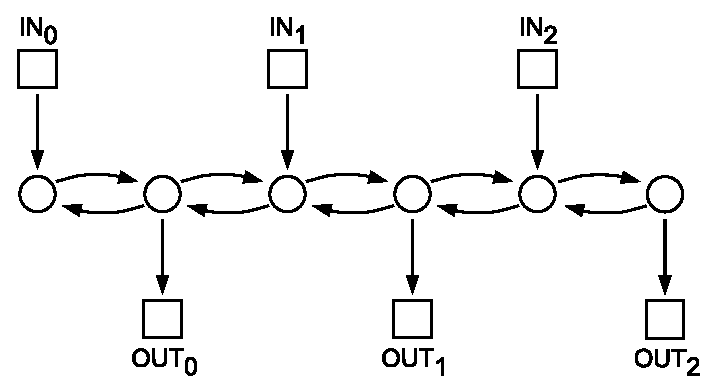
\includegraphics[height=2.0in]{figures/MQ_oct31_network}\\
\end{tabular}
\end{center}

\bparts

\ppart What is the max congestion? \hfill \brule{0.5in}

\begin{solution}
The congestion of the network is at least 3,
  because every path must contain the central switches when $\pi(i) = 2 -
  i$.  The congestion is at most 3, because there are only 3 simple paths
  in total.
\end{solution}

\ppart Give an input/output permutation, $\pi_0$, that forces maximum
  congestion:

\hfill $\pi_0(0) =$ \brule{0.4in}  \qquad $\pi_0(1) =$ \brule{0.4in}
\qquad $\pi_0(2) =$ \brule{0.4in}

\begin{solution}
The permutation $\pi_0$ could be the same as the one specified in
  part (a): $\pi_0(i) = 2-i$.  It could also be $\pi_0(0) = 1$, $\pi_0(1) = 2$, and $\pi_0(2) = 0$.
  In both permutations, all three paths contain the central switch. 
\end{solution}

\ppart\label{minpi} Give an input/output permutation, $\pi_1$, that
allows \emph{minimum} congestion:

\hfill $\pi_1(0) =$ \brule{0.4in}  \qquad $\pi_1(1) =$ \brule{0.4in}
\qquad $\pi_1(2) =$ \brule{0.4in}

\begin{solution}
The permutation is $\pi_1(i) = i$. Each switch has only
  one path going through it, so the congestion is $1$. 
\end{solution}


\ppart What is the latency for the permutation $\pi_1$? (If you could not find $\pi_1$, just choose a permutation and find its latency.)
\hfill\brule{0.5in}

\begin{solution}
\textbf{3}.  This is the latency of
  the (unique) shortest path routing for the permutation in
  part~\eqref{minpi}.  No smaller latency is possible since the minimum
  distance from any input to any output is 3.

\end{solution}
\eparts


\iffalse

{\large
\[
\begin{array}{c|c|c}
%\text{\# switches} &
%\text{switch size} &
\text{diameter} &
\text{latency} &
\text{max congestion} \\ \hline
%\insolutions{6} &
%\insolutions{2 \times 3, 3 \times 2} &
\insolutions{7} &
\insolutions{7} &
\insolutions{3}
\end{array}
\]
}
\fi

\iffalse

  The diameter of a communication net is the largest distance from an input
  to an output.  In this example, the largest distance is from input 0 to
  output 2 of length 7, so the diameter is 7.

  Latency depends on how packets are routed.  If you choose a shortest
  path routing, then the worst I/O pattern (permutation) will be the one
  that maps the maximum distance input to output, so the latency will
  equal the diameter.

  However, a shortest-path routing may be pretty congested, so we're
  usually more interested in the worst latency among the
  minimum-congestion routings.  But in this example, the shortest path
  routing is also the minimum congestion routing, so the latency is any
  case equals the diameter, namely 7.
\fi
  
\end{problem}

%%%%%%%%%%%%%%%%%%%%%%%%%%%%%%%%%%%%%%%%%%%%%%%%%%%%%%%%%%%%%%%%%%%%%
% Problem ends here
%%%%%%%%%%%%%%%%%%%%%%%%%%%%%%%%%%%%%%%%%%%%%%%%%%%%%%%%%%%%%%%%%%%%%
